\documentclass[twoside]{book}

% Packages required by doxygen
\usepackage{fixltx2e}
\usepackage{calc}
\usepackage{doxygen}
\usepackage[export]{adjustbox} % also loads graphicx
\usepackage{graphicx}
\usepackage[utf8]{inputenc}
\usepackage{makeidx}
\usepackage{multicol}
\usepackage{multirow}
\PassOptionsToPackage{warn}{textcomp}
\usepackage{textcomp}
\usepackage[nointegrals]{wasysym}
\usepackage[table]{xcolor}

% Font selection
\usepackage[T1]{fontenc}
\usepackage[scaled=.90]{helvet}
\usepackage{courier}
\usepackage{amssymb}
\usepackage{sectsty}
\renewcommand{\familydefault}{\sfdefault}
\allsectionsfont{%
  \fontseries{bc}\selectfont%
  \color{darkgray}%
}
\renewcommand{\DoxyLabelFont}{%
  \fontseries{bc}\selectfont%
  \color{darkgray}%
}
\newcommand{\+}{\discretionary{\mbox{\scriptsize$\hookleftarrow$}}{}{}}

% Page & text layout
\usepackage{geometry}
\geometry{%
  a4paper,%
  top=2.5cm,%
  bottom=2.5cm,%
  left=2.5cm,%
  right=2.5cm%
}
\tolerance=750
\hfuzz=15pt
\hbadness=750
\setlength{\emergencystretch}{15pt}
\setlength{\parindent}{0cm}
\setlength{\parskip}{3ex plus 2ex minus 2ex}
\makeatletter
\renewcommand{\paragraph}{%
  \@startsection{paragraph}{4}{0ex}{-1.0ex}{1.0ex}{%
    \normalfont\normalsize\bfseries\SS@parafont%
  }%
}
\renewcommand{\subparagraph}{%
  \@startsection{subparagraph}{5}{0ex}{-1.0ex}{1.0ex}{%
    \normalfont\normalsize\bfseries\SS@subparafont%
  }%
}
\makeatother

% Headers & footers
\usepackage{fancyhdr}
\pagestyle{fancyplain}
\fancyhead[LE]{\fancyplain{}{\bfseries\thepage}}
\fancyhead[CE]{\fancyplain{}{}}
\fancyhead[RE]{\fancyplain{}{\bfseries\leftmark}}
\fancyhead[LO]{\fancyplain{}{\bfseries\rightmark}}
\fancyhead[CO]{\fancyplain{}{}}
\fancyhead[RO]{\fancyplain{}{\bfseries\thepage}}
\fancyfoot[LE]{\fancyplain{}{}}
\fancyfoot[CE]{\fancyplain{}{}}
\fancyfoot[RE]{\fancyplain{}{\bfseries\scriptsize Generated by Doxygen }}
\fancyfoot[LO]{\fancyplain{}{\bfseries\scriptsize Generated by Doxygen }}
\fancyfoot[CO]{\fancyplain{}{}}
\fancyfoot[RO]{\fancyplain{}{}}
\renewcommand{\footrulewidth}{0.4pt}
\renewcommand{\chaptermark}[1]{%
  \markboth{#1}{}%
}
\renewcommand{\sectionmark}[1]{%
  \markright{\thesection\ #1}%
}

% Indices & bibliography
\usepackage{natbib}
\usepackage[titles]{tocloft}
\setcounter{tocdepth}{3}
\setcounter{secnumdepth}{5}
\makeindex

% Hyperlinks (required, but should be loaded last)
\usepackage{ifpdf}
\ifpdf
  \usepackage[pdftex,pagebackref=true]{hyperref}
\else
  \usepackage[ps2pdf,pagebackref=true]{hyperref}
\fi
\hypersetup{%
  colorlinks=true,%
  linkcolor=blue,%
  citecolor=blue,%
  unicode%
}

% Custom commands
\newcommand{\clearemptydoublepage}{%
  \newpage{\pagestyle{empty}\cleardoublepage}%
}

\usepackage{caption}
\captionsetup{labelsep=space,justification=centering,font={bf},singlelinecheck=off,skip=4pt,position=top}

%===== C O N T E N T S =====

\begin{document}

% Titlepage & ToC
\hypersetup{pageanchor=false,
             bookmarksnumbered=true,
             pdfencoding=unicode
            }
\pagenumbering{alph}
\begin{titlepage}
\vspace*{7cm}
\begin{center}%
{\Large Final\+Project\+C\+PP }\\
\vspace*{1cm}
{\large Generated by Doxygen 1.8.13}\\
\end{center}
\end{titlepage}
\clearemptydoublepage
\pagenumbering{roman}
\tableofcontents
\clearemptydoublepage
\pagenumbering{arabic}
\hypersetup{pageanchor=true}

%--- Begin generated contents ---
\chapter{Simulador Sistemas Embebidos Robotino}
\label{index}\hypertarget{index}{}\hypertarget{index_autotoc_md0}{}\section{Overview}\label{index_autotoc_md0}
Esta es la documentación del proyecto final de la catedra de Programación Orientada a Objetos en C++.\hypertarget{index_autotoc_md1}{}\section{Objetivos}\label{index_autotoc_md1}


El objetivo es simular la comunicación de 2 arduinos y una raspberry. Ademas, en la raspberry hay un thread corriendo que representa a una camara y envia datos de posición a la raspberry.\hypertarget{index_autotoc_md2}{}\section{Caracteristicas de los SE}\label{index_autotoc_md2}
\hypertarget{index_autotoc_md3}{}\subsection{Raspberry}\label{index_autotoc_md3}

\begin{DoxyItemize}
\item Intercambia mensajes con los Arduinos\+: Recibe mediciones de I\+MU y sensor de distancia y envia seteo de la bomba de agua.
\item Recibe datos del thread de la camara
\end{DoxyItemize}\hypertarget{index_autotoc_md4}{}\subsection{Arduino R}\label{index_autotoc_md4}

\begin{DoxyItemize}
\item Posee una I\+MU que mide aceleraciones en 3 ejes
\item Tiene conectada una bomba de agua a la cual se le setea la tensión
\end{DoxyItemize}\hypertarget{index_autotoc_md5}{}\subsection{Arduino L}\label{index_autotoc_md5}

\begin{DoxyItemize}
\item Tiene un sensor de posición laser
\end{DoxyItemize}\hypertarget{index_autotoc_md6}{}\section{Esquema del programa}\label{index_autotoc_md6}
El programa principal es el archivo \hyperlink{main_8cpp}{main.\+cpp}, donde se disparan los siguientes threads\+:
\begin{DoxyItemize}
\item AR\+: Corre el programa princiapl del Arduino R. En el se toman datos de una I\+MU y se envian a la raspberry. Ademas se leen mensajes que provienen de la raspberry para setear actuadores.
\item AL\+: Corre el programa principal del Arduino L. En el mismo se toman datos de un sensor de distancia y se envian a la raspberry
\item R\+PI\+: Corre el thread de la raspberry pi, dentro del cual se corren lo siguientes threads\+:
\begin{DoxyItemize}
\item Main\+: Corre el programa principal de la raspi, en el mismo se leen datos que provienen de los arduinos y se envian datos para setear los actuadores.
\item Camara\+: Lee datos de posición de la camara y los envia al programa principal de la raspi
\end{DoxyItemize}
\item Quit\+: Revisa si el usuario quiere terminar la simulacion (enter) en caso de querer terminar cierra todos los threads.
\end{DoxyItemize}

Para la generación de los datos de la I\+MU y la camara se leen archivos .txt con los datos de aceleración y posición. En el caso del sensor de distancia, se generan numeros aleatorios para representar la posición medida.\hypertarget{index_autotoc_md7}{}\section{Comunicaciones}\label{index_autotoc_md7}
Para simular la comunicación utilizo queue con strings como elementos donde voy metiendo los mensajes que quiero mandar a otros dispositivos, y el otro dispositivo lee si le corresponde y si le corresponde lo pop, sino no hace nada.

Las siguientes queue se utilizan\+:
\begin{DoxyItemize}
\item queue 1\+: Comunicación entre los arduinos y raspi
\item queue 2\+: Comunicación entre la raspi y la camara
\end{DoxyItemize}\hypertarget{index_autotoc_md8}{}\subsection{Envio de datos}\label{index_autotoc_md8}
A continuación se muestra la estructura de los mensajes de cada dispositivo. \subsubsection*{I\+MU}

!\+D\+AT\+:I\+M\+U\+:xxxx\+:yyyy\+:zzzz\+:\#

\subsubsection*{C\+A\+M\+E\+RA}

!\+D\+AT\+:C\+A\+M\+:xxxx\+:yyyy\+:zzzz\+:\#

\subsubsection*{L\+A\+S\+ER}

!\+D\+AT\+:L\+A\+S\+:xxxx\+:\# 
\chapter{A\+Sdasda}
\label{md__readme}
\Hypertarget{md__readme}
\input{md__readme}
\chapter{Hierarchical Index}
\section{Class Hierarchy}
This inheritance list is sorted roughly, but not completely, alphabetically\+:\begin{DoxyCompactList}
\item \contentsline{section}{Actuator}{\pageref{classActuator}}{}
\begin{DoxyCompactList}
\item \contentsline{section}{Jet\+Pump}{\pageref{classJetPump}}{}
\end{DoxyCompactList}
\item \contentsline{section}{Embeded\+System}{\pageref{classEmbededSystem}}{}
\begin{DoxyCompactList}
\item \contentsline{section}{ArduinoL}{\pageref{classArduinoL}}{}
\item \contentsline{section}{ArduinoR}{\pageref{classArduinoR}}{}
\item \contentsline{section}{Camera}{\pageref{classCamera}}{}
\item \contentsline{section}{Raspi}{\pageref{classRaspi}}{}
\end{DoxyCompactList}
\item \contentsline{section}{Message}{\pageref{classMessage}}{}
\begin{DoxyCompactList}
\item \contentsline{section}{Action\+Msg}{\pageref{classActionMsg}}{}
\item \contentsline{section}{Camera\+Msg}{\pageref{classCameraMsg}}{}
\item \contentsline{section}{Telemetry\+Msg}{\pageref{classTelemetryMsg}}{}
\end{DoxyCompactList}
\item \contentsline{section}{M\+P\+U9250}{\pageref{classMPU9250}}{}
\item \contentsline{section}{Sensor}{\pageref{classSensor}}{}
\begin{DoxyCompactList}
\item \contentsline{section}{Dist\+Sens}{\pageref{classDistSens}}{}
\end{DoxyCompactList}
\item \contentsline{section}{Timer}{\pageref{classTimer}}{}
\end{DoxyCompactList}

\chapter{Class Index}
\section{Class List}
Here are the classes, structs, unions and interfaces with brief descriptions\+:\begin{DoxyCompactList}
\item\contentsline{section}{\hyperlink{classhello}{hello} \\*Simple brief intro  detailed intro }{\pageref{classhello}}{}
\end{DoxyCompactList}

\chapter{File Index}
\section{File List}
Here is a list of all documented files with brief descriptions\+:\begin{DoxyCompactList}
\item\contentsline{section}{\hyperlink{main_8cpp}{main.\+cpp} }{\pageref{main_8cpp}}{}
\item\contentsline{section}{\hyperlink{robsim_8h}{robsim.\+h} }{\pageref{robsim_8h}}{}
\end{DoxyCompactList}

\chapter{Class Documentation}
\hypertarget{class_action_msg}{}\section{Action\+Msg Class Reference}
\label{class_action_msg}\index{Action\+Msg@{Action\+Msg}}


{\ttfamily \#include $<$robsim.\+h$>$}



Inheritance diagram for Action\+Msg\+:
\nopagebreak
\begin{figure}[H]
\begin{center}
\leavevmode
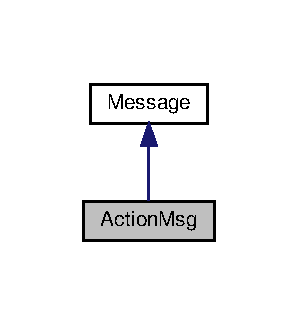
\includegraphics[width=143pt]{class_action_msg__inherit__graph}
\end{center}
\end{figure}


Collaboration diagram for Action\+Msg\+:
\nopagebreak
\begin{figure}[H]
\begin{center}
\leavevmode
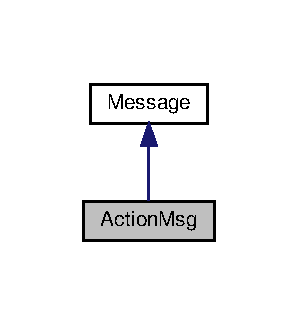
\includegraphics[width=143pt]{class_action_msg__coll__graph}
\end{center}
\end{figure}
\subsection*{Additional Inherited Members}


\subsection{Detailed Description}
Clase mensaje de accion de control 

The documentation for this class was generated from the following file\+:\begin{DoxyCompactItemize}
\item 
\hyperlink{robsim_8h}{robsim.\+h}\end{DoxyCompactItemize}

\hypertarget{class_arduino}{}\section{Arduino Class Reference}
\label{class_arduino}\index{Arduino@{Arduino}}


{\ttfamily \#include $<$robsim.\+h$>$}



\subsection{Detailed Description}
Clase que representa un \hyperlink{class_arduino}{Arduino} 

The documentation for this class was generated from the following file\+:\begin{DoxyCompactItemize}
\item 
\hyperlink{robsim_8h}{robsim.\+h}\end{DoxyCompactItemize}

\hypertarget{class_message}{}\section{Message Class Reference}
\label{class_message}\index{Message@{Message}}


{\ttfamily \#include $<$robsim.\+h$>$}



Inheritance diagram for Message\+:
\nopagebreak
\begin{figure}[H]
\begin{center}
\leavevmode
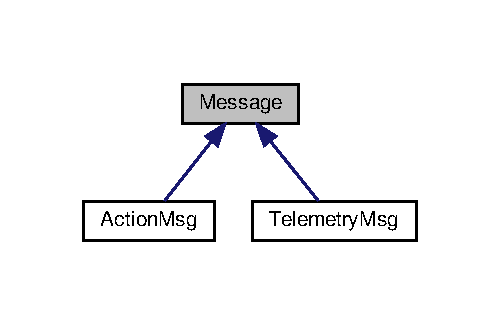
\includegraphics[width=240pt]{class_message__inherit__graph}
\end{center}
\end{figure}
\subsection*{Public Member Functions}
\begin{DoxyCompactItemize}
\item 
\mbox{\Hypertarget{class_message_ab6e3a5a318b80908269f1e9f7110aed9}\label{class_message_ab6e3a5a318b80908269f1e9f7110aed9}} 
void {\bfseries send\+\_\+msg} ()
\item 
\mbox{\Hypertarget{class_message_a74bb67f72c24f9d2367fd82df28b8843}\label{class_message_a74bb67f72c24f9d2367fd82df28b8843}} 
void {\bfseries write\+\_\+msg} ()
\end{DoxyCompactItemize}


\subsection{Detailed Description}
Clase Mensaje 

The documentation for this class was generated from the following file\+:\begin{DoxyCompactItemize}
\item 
\hyperlink{robsim_8h}{robsim.\+h}\end{DoxyCompactItemize}

\hypertarget{class_raspi}{}\section{Raspi Class Reference}
\label{class_raspi}\index{Raspi@{Raspi}}


{\ttfamily \#include $<$robsim.\+h$>$}



\subsection{Detailed Description}
Clase que representa un Raspberry 

The documentation for this class was generated from the following file\+:\begin{DoxyCompactItemize}
\item 
\hyperlink{robsim_8h}{robsim.\+h}\end{DoxyCompactItemize}

\hypertarget{class_telemetry_msg}{}\section{Telemetry\+Msg Class Reference}
\label{class_telemetry_msg}\index{Telemetry\+Msg@{Telemetry\+Msg}}


{\ttfamily \#include $<$robsim.\+h$>$}



Inheritance diagram for Telemetry\+Msg\+:
\nopagebreak
\begin{figure}[H]
\begin{center}
\leavevmode
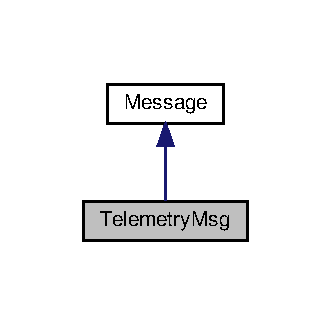
\includegraphics[width=159pt]{class_telemetry_msg__inherit__graph}
\end{center}
\end{figure}


Collaboration diagram for Telemetry\+Msg\+:
\nopagebreak
\begin{figure}[H]
\begin{center}
\leavevmode
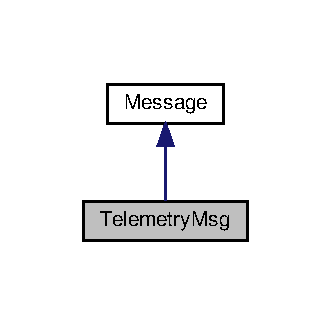
\includegraphics[width=159pt]{class_telemetry_msg__coll__graph}
\end{center}
\end{figure}
\subsection*{Additional Inherited Members}


\subsection{Detailed Description}
Clase mensaje de telemetria 

The documentation for this class was generated from the following file\+:\begin{DoxyCompactItemize}
\item 
\hyperlink{robsim_8h}{robsim.\+h}\end{DoxyCompactItemize}

\chapter{File Documentation}
\hypertarget{main_8cpp}{}\section{main.\+cpp File Reference}
\label{main_8cpp}\index{main.\+cpp@{main.\+cpp}}
{\ttfamily \#include $<$iostream$>$}\newline
Include dependency graph for main.\+cpp\+:\nopagebreak
\begin{figure}[H]
\begin{center}
\leavevmode
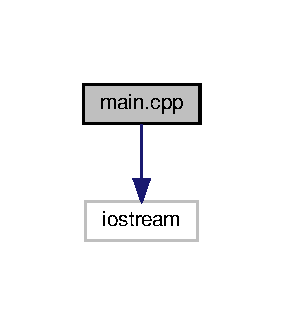
\includegraphics[width=136pt]{main_8cpp__incl}
\end{center}
\end{figure}
\subsection*{Functions}
\begin{DoxyCompactItemize}
\item 
\mbox{\Hypertarget{main_8cpp_ae66f6b31b5ad750f1fe042a706a4e3d4}\label{main_8cpp_ae66f6b31b5ad750f1fe042a706a4e3d4}} 
int {\bfseries main} ()
\end{DoxyCompactItemize}

\hypertarget{robsim_8h}{}\section{src/robsim.h File Reference}
\label{robsim_8h}\index{src/robsim.\+h@{src/robsim.\+h}}
{\ttfamily \#include $<$queue$>$}\newline
{\ttfamily \#include \char`\"{}sensors.\+h\char`\"{}}\newline
{\ttfamily \#include $<$sys/time.\+h$>$}\newline
Include dependency graph for robsim.\+h\+:\nopagebreak
\begin{figure}[H]
\begin{center}
\leavevmode
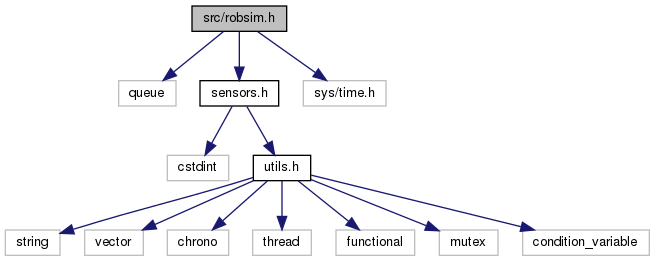
\includegraphics[width=350pt]{robsim_8h__incl}
\end{center}
\end{figure}
This graph shows which files directly or indirectly include this file\+:\nopagebreak
\begin{figure}[H]
\begin{center}
\leavevmode
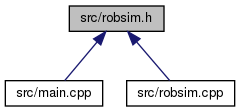
\includegraphics[width=252pt]{robsim_8h__dep__incl}
\end{center}
\end{figure}
\subsection*{Classes}
\begin{DoxyCompactItemize}
\item 
class \hyperlink{classEmbededSystem}{Embeded\+System}
\begin{DoxyCompactList}\small\item\em a Clase base Sistema embebido Tiene como metodo virtual puro el main de los SE \end{DoxyCompactList}\item 
class \hyperlink{classArduinoR}{ArduinoR}
\begin{DoxyCompactList}\small\item\em Clase que representa el Arduino dedicado al sistema 1 El metodo main es el bucle infinito del SE Hereda de la clase Sistema Embebido. \end{DoxyCompactList}\item 
class \hyperlink{classArduinoL}{ArduinoL}
\begin{DoxyCompactList}\small\item\em Clase que representa el Arduino dedicado al sistema 2 El metodo main es el bucle infinito del SE. \end{DoxyCompactList}\item 
class \hyperlink{classRaspi}{Raspi}
\begin{DoxyCompactList}\small\item\em Clase que representa la Raspberry El metodo main es el bucle infinito del SE. \end{DoxyCompactList}\item 
class \hyperlink{classCamera}{Camera}
\begin{DoxyCompactList}\small\item\em Clase que representa la camara El metodo main es el bucle infinito del SE. \end{DoxyCompactList}\item 
class \hyperlink{classActuator}{Actuator}
\begin{DoxyCompactList}\small\item\em Clase base actuadores. \end{DoxyCompactList}\item 
class \hyperlink{classJetPump}{Jet\+Pump}
\begin{DoxyCompactList}\small\item\em Clase \hyperlink{classJetPump}{Jet\+Pump}. \end{DoxyCompactList}\item 
class \hyperlink{classSensor}{Sensor}
\begin{DoxyCompactList}\small\item\em Clase base sensores. \end{DoxyCompactList}\item 
class \hyperlink{classDistSens}{Dist\+Sens}
\begin{DoxyCompactList}\small\item\em Clase que representa el sensor de dist. \end{DoxyCompactList}\item 
class \hyperlink{classMessage}{Message}
\begin{DoxyCompactList}\small\item\em Clase Mensaje. \end{DoxyCompactList}\item 
class \hyperlink{classTelemetryMsg}{Telemetry\+Msg}
\begin{DoxyCompactList}\small\item\em Clase mensaje de telemetria. \end{DoxyCompactList}\item 
class \hyperlink{classActionMsg}{Action\+Msg}
\begin{DoxyCompactList}\small\item\em Clase mensaje de accion de control. \end{DoxyCompactList}\item 
class \hyperlink{classCameraMsg}{Camera\+Msg}
\begin{DoxyCompactList}\small\item\em Clase mensaje de camara. \end{DoxyCompactList}\end{DoxyCompactItemize}
\subsection*{Macros}
\begin{DoxyCompactItemize}
\item 
\#define \hyperlink{robsim_8h_a6a7d0aa2f8672b5fd4207bf9a4d2912d}{M\+S\+G\+\_\+\+T\+E\+L\+E\+M\+E\+T\+RY}~\hyperlink{classMessage_a1c65ab3f02ba5b175f583f9d275ecf2babb3d2d909c73fe49800949a344775f8b}{Message\+::\+Type\+::\+T\+E\+L\+E\+M\+E\+T\+RY}
\item 
\#define \hyperlink{robsim_8h_add686b3cb16e812ad19e05944997c2a7}{M\+S\+G\+\_\+\+A\+C\+T\+I\+ON}~\hyperlink{classMessage_a1c65ab3f02ba5b175f583f9d275ecf2bae58a1b00942e66d8b4abc960da7877ab}{Message\+::\+Type\+::\+A\+C\+T\+I\+ON}
\item 
\#define \hyperlink{robsim_8h_ad066d2f092a3d1bb49aca1f9524c66c3}{M\+S\+G\+\_\+\+C\+A\+M\+E\+RA}~\hyperlink{classMessage_a1c65ab3f02ba5b175f583f9d275ecf2baddf0d6b21537d984fea6544f58101fa8}{Message\+::\+Type\+::\+C\+A\+M\+E\+RA}
\end{DoxyCompactItemize}
\subsection*{Functions}
\begin{DoxyCompactItemize}
\item 
int \hyperlink{robsim_8h_abfd055405fc0db9a96a29057436d7e6b}{time\+\_\+falt\+\_\+next\+\_\+interv\+\_\+ms} (struct timeval $\ast$t0, int n, double dt)
\begin{DoxyCompactList}\small\item\em Calcula el tiempo faltante para el siguiente intervalo. \end{DoxyCompactList}\item 
void \hyperlink{robsim_8h_ae9bdf1cf8a02cfad30e904f75ede4f4e}{espera\+\_\+siguiente\+\_\+intervalo} (struct timeval $\ast$t0, int n, double dt)
\begin{DoxyCompactList}\small\item\em Función bloqueante que espera hasta el siguiente intervalor. \end{DoxyCompactList}\end{DoxyCompactItemize}


\subsection{Detailed Description}
\begin{DoxyAuthor}{Author}
Francisco Ortiz 
\end{DoxyAuthor}


\subsection{Macro Definition Documentation}
\mbox{\Hypertarget{robsim_8h_add686b3cb16e812ad19e05944997c2a7}\label{robsim_8h_add686b3cb16e812ad19e05944997c2a7}} 
\index{robsim.\+h@{robsim.\+h}!M\+S\+G\+\_\+\+A\+C\+T\+I\+ON@{M\+S\+G\+\_\+\+A\+C\+T\+I\+ON}}
\index{M\+S\+G\+\_\+\+A\+C\+T\+I\+ON@{M\+S\+G\+\_\+\+A\+C\+T\+I\+ON}!robsim.\+h@{robsim.\+h}}
\subsubsection{\texorpdfstring{M\+S\+G\+\_\+\+A\+C\+T\+I\+ON}{MSG\_ACTION}}
{\footnotesize\ttfamily \#define M\+S\+G\+\_\+\+A\+C\+T\+I\+ON~\hyperlink{classMessage_a1c65ab3f02ba5b175f583f9d275ecf2bae58a1b00942e66d8b4abc960da7877ab}{Message\+::\+Type\+::\+A\+C\+T\+I\+ON}}



Definition at line 15 of file robsim.\+h.

\mbox{\Hypertarget{robsim_8h_ad066d2f092a3d1bb49aca1f9524c66c3}\label{robsim_8h_ad066d2f092a3d1bb49aca1f9524c66c3}} 
\index{robsim.\+h@{robsim.\+h}!M\+S\+G\+\_\+\+C\+A\+M\+E\+RA@{M\+S\+G\+\_\+\+C\+A\+M\+E\+RA}}
\index{M\+S\+G\+\_\+\+C\+A\+M\+E\+RA@{M\+S\+G\+\_\+\+C\+A\+M\+E\+RA}!robsim.\+h@{robsim.\+h}}
\subsubsection{\texorpdfstring{M\+S\+G\+\_\+\+C\+A\+M\+E\+RA}{MSG\_CAMERA}}
{\footnotesize\ttfamily \#define M\+S\+G\+\_\+\+C\+A\+M\+E\+RA~\hyperlink{classMessage_a1c65ab3f02ba5b175f583f9d275ecf2baddf0d6b21537d984fea6544f58101fa8}{Message\+::\+Type\+::\+C\+A\+M\+E\+RA}}



Definition at line 16 of file robsim.\+h.

\mbox{\Hypertarget{robsim_8h_a6a7d0aa2f8672b5fd4207bf9a4d2912d}\label{robsim_8h_a6a7d0aa2f8672b5fd4207bf9a4d2912d}} 
\index{robsim.\+h@{robsim.\+h}!M\+S\+G\+\_\+\+T\+E\+L\+E\+M\+E\+T\+RY@{M\+S\+G\+\_\+\+T\+E\+L\+E\+M\+E\+T\+RY}}
\index{M\+S\+G\+\_\+\+T\+E\+L\+E\+M\+E\+T\+RY@{M\+S\+G\+\_\+\+T\+E\+L\+E\+M\+E\+T\+RY}!robsim.\+h@{robsim.\+h}}
\subsubsection{\texorpdfstring{M\+S\+G\+\_\+\+T\+E\+L\+E\+M\+E\+T\+RY}{MSG\_TELEMETRY}}
{\footnotesize\ttfamily \#define M\+S\+G\+\_\+\+T\+E\+L\+E\+M\+E\+T\+RY~\hyperlink{classMessage_a1c65ab3f02ba5b175f583f9d275ecf2babb3d2d909c73fe49800949a344775f8b}{Message\+::\+Type\+::\+T\+E\+L\+E\+M\+E\+T\+RY}}



Definition at line 14 of file robsim.\+h.



\subsection{Function Documentation}
\mbox{\Hypertarget{robsim_8h_ae9bdf1cf8a02cfad30e904f75ede4f4e}\label{robsim_8h_ae9bdf1cf8a02cfad30e904f75ede4f4e}} 
\index{robsim.\+h@{robsim.\+h}!espera\+\_\+siguiente\+\_\+intervalo@{espera\+\_\+siguiente\+\_\+intervalo}}
\index{espera\+\_\+siguiente\+\_\+intervalo@{espera\+\_\+siguiente\+\_\+intervalo}!robsim.\+h@{robsim.\+h}}
\subsubsection{\texorpdfstring{espera\+\_\+siguiente\+\_\+intervalo()}{espera\_siguiente\_intervalo()}}
{\footnotesize\ttfamily void espera\+\_\+siguiente\+\_\+intervalo (\begin{DoxyParamCaption}\item[{struct timeval $\ast$}]{t0,  }\item[{int}]{n,  }\item[{double}]{dt }\end{DoxyParamCaption})}



Función bloqueante que espera hasta el siguiente intervalor. 


\begin{DoxyParams}[1]{Parameters}
\mbox{\tt in}  & {\em $\ast$t0} & puntero a timeval con el tiempo incial del experimento \\
\hline
\mbox{\tt in}  & {\em n} & numero de intervalo \\
\hline
\mbox{\tt in}  & {\em dt} & paso de tiempo \\
\hline
\end{DoxyParams}


Definition at line 34 of file robsim.\+cpp.

\mbox{\Hypertarget{robsim_8h_abfd055405fc0db9a96a29057436d7e6b}\label{robsim_8h_abfd055405fc0db9a96a29057436d7e6b}} 
\index{robsim.\+h@{robsim.\+h}!time\+\_\+falt\+\_\+next\+\_\+interv\+\_\+ms@{time\+\_\+falt\+\_\+next\+\_\+interv\+\_\+ms}}
\index{time\+\_\+falt\+\_\+next\+\_\+interv\+\_\+ms@{time\+\_\+falt\+\_\+next\+\_\+interv\+\_\+ms}!robsim.\+h@{robsim.\+h}}
\subsubsection{\texorpdfstring{time\+\_\+falt\+\_\+next\+\_\+interv\+\_\+ms()}{time\_falt\_next\_interv\_ms()}}
{\footnotesize\ttfamily int time\+\_\+falt\+\_\+next\+\_\+interv\+\_\+ms (\begin{DoxyParamCaption}\item[{struct timeval $\ast$}]{t0,  }\item[{int}]{n,  }\item[{double}]{dt }\end{DoxyParamCaption})}



Calcula el tiempo faltante para el siguiente intervalo. 


\begin{DoxyParams}[1]{Parameters}
\mbox{\tt in}  & {\em $\ast$t0} & puntero a timeval con el tiempo incial del experimento \\
\hline
\mbox{\tt in}  & {\em n} & numero de intervalor \\
\hline
\mbox{\tt in}  & {\em dt} & paso de tiempo\\
\hline
\end{DoxyParams}
\begin{DoxyReturn}{Returns}
Tiempo en ms hasta el intervalo n 
\end{DoxyReturn}


Definition at line 25 of file robsim.\+cpp.


%--- End generated contents ---

% Index
\backmatter
\newpage
\phantomsection
\clearemptydoublepage
\addcontentsline{toc}{chapter}{Index}
\printindex

\end{document}
